\documentclass[a4paper,12pt]{article}
\usepackage[english]{babel}
\usepackage[right=2.5cm,left=2.5cm,top=2cm,bottom=2cm]{geometry}
\usepackage[utf8]{inputenc}
\usepackage{amsmath}
\usepackage{amssymb}
\usepackage{mathrsfs}
\usepackage{latexsym}
\usepackage{dsfont}
\usepackage{amsfonts}
\usepackage{array}
\usepackage{hyperref}
%\usepackage{fancyhdr}
\usepackage{xcolor}
%\pagestyle{fancy}
\usepackage{blindtext}
\usepackage{graphicx}
\usepackage{enumerate}
\usepackage{enumitem}
\usepackage{caption}
\usepackage[left]{sidecap}
\usepackage[]{float}
\usepackage{multirow}
\usepackage[style=apa]{biblatex}
\bibliography{bio}
\begin{document}

\begin{titlepage}
\centering
{\bfseries\LARGE {Art\'iculo cient\'ifico}\par}
\vspace{1cm}
{\scshape\Large {Tarea 6. & Publiaciones cient\'ificas} \par}
\vspace{3cm}
{\scshape\Huge\textbf {Anthropogenic emission is the main contributor to the rise of atmospheric methane during 1993–2017} \par}
\vspace{3cm}
{\itshape\Large\textbf {Trabajo en equipo}\par}
\vfill
{\Large\textbf {Members:} \par}

\begin{itemize}
\begin{center}
    \item {\Large{Jared Emmanuel Aguirre Vera}}
    \item {\Large{Luis Fernando Sotomayor Garcia}}
    \item {\Large{Karla Cecilia Valeria Rios Lara}} 
    \item {\Large{Esteban Villa Rosas}}
\end{center}
\end{itemize}
%{\Large Sotomayor Garcia Luis Fernando\par}
\vfill
{\Large November 20, 2022. \par}
\end{titlepage}



\begin{center}

{\Huge{{\textbf{Anthropogenic emission is the main contributor to the rise of atmospheric methane during 1993–2017}}}}

\end{center}

\small{Zhen Zhang, Benjamin Poulter, Sara Knox, Ann Stavert, Gavin McNicol, Etienne Fluet-Chouinard, Aryeh Feinberg, Yuanhong Zhao, Philippe Bousquet, Josep G Canadell, Anita Ganesan, Gustaf Hugelius, George Hurtt, Robert B Jackson, Prabir K Patra, Marielle Saunois, Lena Höglund-Isaksson, Chunlin Huang, Abhishek Chatterjee, Xin Li}\\

\small{National Science Review, Volume 9, Issue 5, May 2022, nwab200}

\small{\textbf{Published:} 11 November 2021}

\begin{abstract}
    Atmospheric methane $(CH_4)$ concentrations have shown a puzzling resumption in growth since 2007 following a period of stabilization from 2000 to 2006. Multiple hypotheses have been proposed to explain the temporal variations in $CH_4$ growth, and attribute the rise of atmospheric $CH_4$ either to increases in emissions from fossil fuel activities, agriculture and natural wetlands, or to a decrease in the atmospheric chemical sink. Here, we use a comprehensive ensemble of $CH_4$ source estimates and isotopic $\delta^{13}C-CH_4$ source signature data to show that the resumption of $CH_4$ growth is most likely due to increased anthropogenic emissions. Our emission scenarios that have the fewest biases with respect to isotopic composition suggest that the agriculture, landfill and waste sectors were responsible for $53 \pm 13\%$ of the renewed growth over the period 2007–2017 compared to 2000–2006; industrial fossil fuel sources explained an additional $34 \pm 24\%$, and wetland sources contributed the least at $13 \pm 9\%$. The hypothesis that a large increase in emissions from natural wetlands drove the decrease in atmospheric $\delta^{13}C-CH_4$ values cannot be reconciled with current process-based wetland $CH_4$ models. This finding suggests the need for increased wetland measurements to better understand the contemporary and future role of wetlands in the rise of atmospheric methane and climate feedback. Our findings highlight the predominant role of anthropogenic activities in driving the growth of atmospheric $CH_4$ concentrations.
\end{abstract}

\section*{\textbf{\textsc{\Large{\underline{INTRODUCTION}}}}}

\small{Stabilizing atmospheric methane $CH_{4}$ emissions from anthropogenic activities is a critical component of climate change mitigation. The atmospheric $CH_{4}$ concentration has increased $\sim$2.5-fold from 731 ppb (parts per billion) in 1750 (pre-industrial reference year ) to 1890 ppb in 2020. Meanwhile, over the past century, atmospheric $\delta ^1^3C-CH_{4}$ values increased from $\sim−49.0\%$ in 1912 to $−47.2\%$in 2007 due to increasing emissions of isotopically $^1^3$C-enriched (i.e. isotopically heavy) fossil fuels. Despite the importance of understanding the temporal changes in atmospheric $CH_{4}$, the drivers of changes in the growth rate of atmospheric $CH_{4}$ over recent decades remain poorly understood. The increase in atmospheric $CH_{4}$ slowed in the early 1990s and was followed by a so-called stabilization period during 2000–2006. Since 2007, global atmospheric $CH_{4}$ concentrations have begun to rise again, accompanied by a decline in $\delta ^1^3C-CH_{4}$ values from $−47.2\%$ in 2007 to $−47.4\%$ in 2017. The cause of this change has been studied recently using atmospheric inversion models, atmospheric box models and emission inventories. These studies have arrived at divergent and even conflicting conclusions, citing increasing emissions of $CH_{4}$ from fossil fuels, agriculture, wetlands and/or decreased hydroxyl radicals (OH) as main drivers due to different measurements, methodologies and time periods considered (see Materials and Methods). Such discrepancies highlight the need to reconcile our understanding of the drivers of growth in atmospheric $CH_{4}$ in order to design mitigation policies.}
\\\\
\small{Sources of the global $CH_{4}$ budget are mainly determined by three broadly defined groups: (i) thermogenic sources from industrial fossil fuel (e.g. coal, oil and natural gas; IFF$CH_{4}$) and geological sources (GEO$CH_{4}$); (ii) biogenic sources from livestock, rice agriculture, landfills and waste (AGW$CH_{4}$), and natural wetlands (WET$CH_{4}$); and (iii) pyrogenic sources from wildfires and biomass burning (BB$CH_{4}$). The primary sink for $CH_{4}$ is reactions with tropospheric OH, soil microbial uptake and a small contribution from tropospheric chlorine reactions, which affect the isotopic compositions. The shift of the trend in atmospheric $\delta ^1^3C-CH_{4}$ values towards more $^1^3C$-depleted (i.e. isotopically light) compositions suggests a higher dominance of isotopically light biogenic emissions in the global $CH_{4}$ budget. This hypothesis has been supported by recent process-based and inversion modeling, which points to either a systematic underestimation of AGW$CH_{4}$ or a large increase in WET$CH_{4}$. In contrast, there are large differences in the rate of change across inventory-based estimates of industrial fossil fuel source activity IFF$CH_{4}$, as well as substantial underestimates in some regions and overestimates in other regions. Globally, studies suggest that BB$CH_{4}$ has been declining, with fire $CH_{4}$ emissions associated with an isotopically enriched signature, thus providing room in the isotopic budget for an increase in fossil fuel sources. GEO$CH_{4}$, which is often co-located with the fossil fuel industry, is suggested to be largely overestimated by recent studies, indicating a potentially larger role of IFF$CH_{4}$ in affecting the global $CH_{4}$ budget given its underestimated share of the total $CH_{4}$ source.}
\\\\
\small{OH oxidation in the troposphere is the main $CH_{4}$ sink, and reactions with chlorine (Cl), stratospheric sinks and soil removal are small-magnitude sinks. Substantial difficulties remain in quantifying $CH_{4}$ sinks, especially the main chemical sink for  $CH_{4}$, tropospheric OH. OH plays a significant but ambiguous role in driving the observed atmospheric trend; it is difficult to estimate due to its complicated chemistry, i.e. non-linear chemical feedback and short lifetime. For example, estimates of interannual variability (IAV) in global mean OH are significantly higher in the empirical box-model estimates that use CO and methylchloroform (MCF) constraints than estimates based on chemical transport models (Fig. S1). Although there are debates on the potential biases in the box-model-based OH due to ignorance of complex spatial heterogeneity in OH and transport, the uncertainties in OH trends and variability are likely large enough to explain any potential $CH_{4}$ growth scenarios. In addition, the trends in OH exert isotopic leverage on atmospheric δ13C-CH4 values via the kinetic fractionation effect, such that increasing OH increases the atmospheric $\delta ^1^3C-CH_{4}$ value by OH reacting with more  $1^2^CH_{4}$. Therefore, it is of interest to investigate hypotheses regarding $CH_{4}$ sources with atmospheric $\delta ^1^3C-CH_{4}$ observations while assuming that these sources can reproduce the atmospheric records with varying OH.}
\\\\
\small{A thorough investigation of these hypotheses in a clearly defined framework is essential to help resolve the unexplained change in the growth rate of atmospheric $CH_{4}$. Here, we use an isotopic mass balance approach to attribute drivers of the growth rate of atmospheric $CH_{4}$ using a large ensemble of scenarios to represent different combinations of emission hypotheses (denoted emission scenarios, see Materials and Methods) from a comprehensive set of updated bottom-up estimates representing anthropogenic emission inventories and spatially explicit signatures for major $CH_{4}$ sources. Each emission scenario is composed of a time series of sectoral $CH_{4}$ fluxes and their hemispheric emission-weighted $\delta ^1^3C-CH_{4}$ values. A globally representative database and spatially resolved distributions of $\delta ^1^3C-CH_{4}$ values for the major $CH_{4}$ sources were used to evaluate the temporal and regional variability in observed $\delta ^1^3C-CH_{4}$values. Monte Carlo techniques were applied to explore the uncertainty in $\delta ^1^3C-CH_{4}$ estimates with full consideration of the spatial heterogeneity in $CH_{4}$ sources and their $\delta ^1^3C-CH_{4}$ signatures. Scenario-specific parameters for the time series of the $CH_{4}$ removal rate driven by OH variations and run-specific $1^3 CH_{4}$ fractionation factors were derived by inverting an atmospheric two-box model (see Methods and Supplementary Data). We then evaluated the emission scenarios against observed $\delta ^1^3C-CH_{4}$ values for 1993–2017 by running the two-box model in the forward mode. To test the hypothesis of a large increase from wetland $CH_{4}$ emissions, the idealized wetland scenarios (i.e. without process-based constraint) were then calculated to reproduce the temporal pattern of $\delta ^1^3C-CH_{4}$. The comparison against atmospheric isotopic observations allowed us to select the most likely set of emission scenarios, which are defined as the first percentile cut-off of the lowest mean squared difference (MSD) in simulated $\delta ^1^3C-CH_{4}$ values.}


\section*{\textbf{\textsc{\Large{\underline{RESULTS AND DISCUSSION}}}}}


\subsection*{\textbf{\textsc{\large{Temporal variations in the atmospheric $CH_{4}$ concentration and its $\delta^{13}$$C-CH_{4}$ value}}}}\\

\small{The ensemble simulations for the 96 emission scenarios(4IFF$_{CH4}$ x3$AGW_{CH4}$ X2WET$_{CH4}$ X2BB$_{CH4}$ X2GEO$_{CH4}$)reproduced the observed atmospheric $CH_{4}$ concentration (Fig. \ref{fig1:my_label}A) using the corresponding optimized time series of OH derived from running the box model in inverse mode (Fig. S1). We accounted for the uncertainty in source signatures of $\delta^{13}$$C-CH_{4}$ by resampling 1000 sets of $\delta^{13}$$C-CH_{4}$ signature time series for each emission scenario (n=96 × 1000), which resulted in a wide range of modeled atmospheric $\delta^{13}$$C-CH_{4}$ values with some closely reproducing the observations. However, most emission scenarios tended to generate more enriched $\delta^{13}$$C-CH_{4}$ trends for 1993–2017, suggesting that existing bottom-up inventories overestimate the increase in IFF$_{CH4}$ during the study period, especially during slowdown and stagnation periods (Fig. \ref{fig1:my_label}B). Furthermore, to balance the rise in $CH_{4}$ sources, the increases in OH levels also led to positive trends in atmospheric $\delta^{13}$$C-CH_{4}$ values during these two periods (Fig. S1). Note that the large increase in coal-related emissions since 2003 has increased the $\delta^{13}$$C-CH_{4}$ values of the sources, which contribute to the divergence between the model and observations. The timing of this divergence is consistent with a rapid increase in methane emissions from China (mainly coal emissions) as reported by the inventories [23] and inversions [39]. For most of the emission scenarios, the estimated temporal variations in OH for 1993–2017 fall within the $1-\sigma$ range of the Bayesian inversion from Ref. [14] and are in good agreement with Ref. [35] for the post-2000 period. The EDGARv4.2-based emission scenarios have the largest mismatch with the inversion-based OH anomaly (relative to a global mean concentration of $1e^{6}$ molecules $(molec)/cm^{3})$confirming the known higher bias in EDGARv4.2 than in other inventories (Fig. S2).}\\\\

\begin{figure}[H]
    \caption{}
    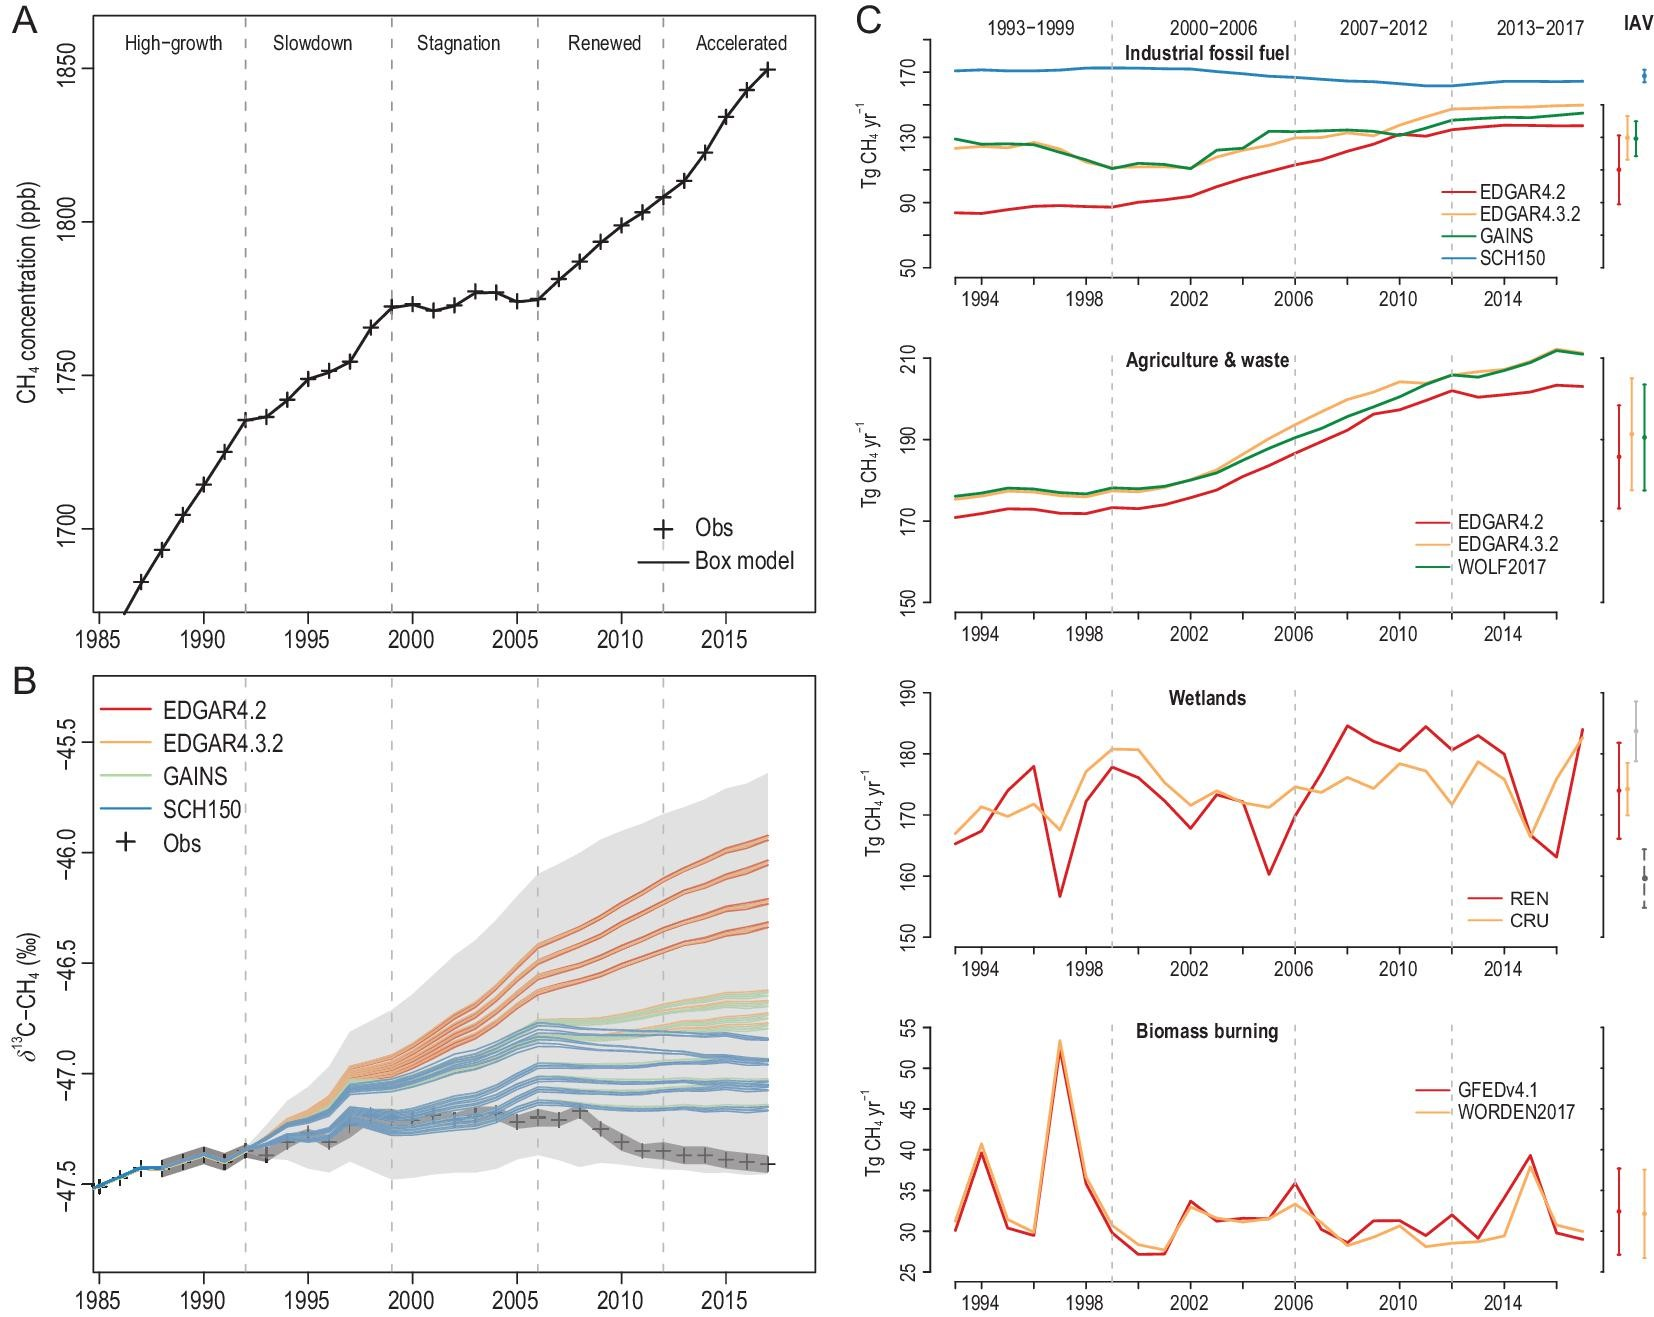
\includegraphics[width=\textwidth, height=9cm]{figure 1..jpeg}
    \label{fig1:my_label}





\textit{\scriptsize{Simulated global atmospheric $CH_{4}$ concentration, $\delta^{13}$$C-CH_{4}$ values and bottom-up estimates of major $CH_{4}$ sources. (A) Simulated atmospheric $CH_{4}$ concentration (black solid line) from all emission scenarios exactly reproducing the observed $CH_{4}$ records (cross dots). The ensemble simulations of the box model were run in forward mode with prescribed $\delta^{13}$$C-CH_{4}$ variations from emission scenarios using $OH$ time series derived from inverse mode (Fig. S1). (B) Simulated ensemble mean $\delta^{13}$$C-CH_{4}$ values (colored solid lines) for emission scenarios grouped by industrial fossil fuel inventories (EDGARv4.2, EDGARv4.3.2, GAINS and SCH150) in comparison to the observed global mean $\delta^{13}$$C-CH_{4}$ (cross). The uncertainty range of ensemble simulations (n = 96000) and $1-\sigma$ uncertainty of the observations are shown as light gray areas and dark gray areas, respectively.(C) Time series of annual total emissions for major sources. The interannual variability $(1-\sigma)$ in $CH_{4}$  for each individual bottom-up estimate is shown at the right of the plot. Note that for the wetland category, the dashed bars represent two independent estimates from a bottom-up ensemble of wetland models [40] for 2000–2012 (light gray) and WetCHARTs [41] (dark gray) for 2001–2015.}}
\end{figure}
\\\\
\small{The time series of $CH_{4}$ sources for 1993–2017 (Fig. \ref{fig1:my_label}C) suggests that decadal-scale variations in atmospheric $CH_{4}$ are dominated by anthropogenic emissions from both agricultural and fossil fuel activities. However, there is high uncertainty across IFF$_{CH4}$ inventories, with a sizable $(>40Tg CH_{4}yr^{-1})$ difference in magnitude and a large difference in temporal trends between inventories (i.e. EDGARv4.2, EDGARv4.3.2 and GAINS) and an atmospheric-observation-constrained approach (i.e. SCH150, which hypothesizes that IFF$_{CH4}$ is underestimated but does not increase over time). The temporal variation in AGW$_{CH4}$ exhibits a lower discrepancy than IFF$_{CH4}$ in the inventories, whereas WET$_{CH4}$ and BB$_{CH4}$ are more constrained. The IAV and magnitude of our estimates for WET$_{CH4}$, calculated using the process-based model LPJ-wsl, are comparable to the ensemble mean of multiple wetland models [40] and a global wetland $CH_{4}$ emission model ensemble for use in atmospheric chemical transport models (WetCHARTs) [41]. The wetland $CH_{4}$ estimates derived from driving the wetland model with a ground-measurement-based meteorological dataset from the Climate Research Unit (CRU) yield a small increase $(<1Tg CH_{4}yr^{-1})$, whereas the same model with climate reanalysis (REN) has an $ \sim7.3 TgCH_{4}$ step increase from tropical wetlands between 2000–2006 and 2007–2017 [22].}


\subsection*{\textbf{\textsc{\large{Evaluations of proposed $CH_{4}$ hypotheses using emission scenarios}}}}\\

\small{Figure \ref{fig2:my_label}A shows the distribution of residual bias in the individual box model simulations in terms of how they reproduce the observed $\delta^{13}$$C-CH_{4}$ values. In the Taylor diagram [42] the global average $\delta^{13}$$C-CH_{4}$ values of the sources before fractionation by chemical sinks range from $-53\% to -55\%$ over 1993–2017, and a correlation coefficient lower than 0.6 is obtained for all of the simulations for 1993–2017. The low agreement suggests that the biases in the inventories and the wetland models contribute to the discrepancies in reproducing the $\delta^{13}$$C-CH_{4}$ , which is likely due to the overestimated increase in inventories, especially the coal emission that has a relatively heavy isotopic signature, as found by previous atmospheric inversion studies [16]. In addition, some of the simulations can reproduce similar IAV in atmospheric $\delta^{13}$$C-CH_{4}$ values with root mean square errors (RMSEs) from $0.05\%$ to $0.5\%$, but $\sim 85\%$ of simulations tend to produce higher IAV than observed. Although the global average $\delta^{13}$$C-CH_{4}$ value was regarded as observational ‘truth’, this reference has an uncertainty of $0.04\%$, attributed to variability in measurements across all the stations and uncertainty from scale conversions between networks [43].}

\begin{figure}[H]
    \caption{}
    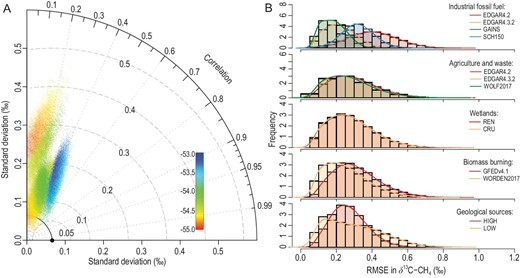
\includegraphics[width=\textwidth, height=9cm]{figure 2.jpeg}
    \label{fig2:my_label}



\textit{\scriptsize{Performance of emission scenarios in simulating atmospheric $\delta^{13}$$C-CH_{4}$.(A) Taylor diagram illustrating the similarity between individual time series from the 96000 simulations of different emission scenarios (colored dots) to the observed atmospheric $\delta^{13}$$C-CH_{4}$ for 1993–2017. The black solid dot refers to the observed global average $\delta^{13}$$C-CH_{4}$ for 1993–2017. Each dot symbol indicates the correlation value (angle), the standard deviation (SD, radial distance to the origin point) and the root mean square error (RMSE, distance to the black solid dot), with different colors representing the mean global average $\delta^{13}$$C-CH_{4}$ value of the source. (B) Histograms of RMSE between simulated $\delta^{13}$$C-CH_{4}$ values and observations grouped by bottom-up estimates with different colors for major $CH_{4}$ source categories. The solid lines represent the fitted density distribution after spline smoothing.}}
\end{figure}
\\\\
\small{The density distributions of RMSEs grouped by different bottom-up $CH_{4}$ estimates show the divergent performance of emission scenarios in reproducing observed atmospheric $\delta^{13}$$C-CH_{4}$ values (Fig. \ref{fig2:my_label}B). Among the four IFF$_{CH4}$ inventories, $80\%$ of the simulations using EDGARv4.2 generated more positive trends of $\delta^{13}$$C-CH_{4}$ values than the other three inventories, with no EDGARv4.2-based runs located in the most likely set of emission scenarios (Fig. S3). This result corroborates previous studies that also suggest that EDGARv4.2 tends to overestimate fossil fuel growth [44]. The more recent EDGARv4.3.2 has been improved, with $95\%$ of the simulations located within the RMSE range from $0.1\%$ to $0.3\%$, mainly due to improved emission factors and revised statistics of $CH_{4}$ sectors [23]. SCH150 produces lower agreement than EDGARv4.3.2 partly due to the low IAV of SCH150, as SCH150 focuses on the long-term trends in IFF$_{CH4}$. The GAINS inventories generated better performance:$78\%$ of the simulations in the first percentile of MSD are based on GAINS IFF$_{CH4}$. Note that this does not rule out the IFF$_{CH4}$ scenarios that have flat or insignificant trends (e.g. SCH150), as $^{13}C-enriched BB_{CH4}$ estimates in this study show declining trends over recent years, which would allow for compensation by increasing emissions from IFF$_{CH4}$ to meet the decreasing atmospheric $\delta^{13}$$C-CH_{4}$ values. Generally, IFF$_{CH4}$ has a more pronounced impact in determining the past trends in $\delta^{13}$$C-CH_{4}$ changes than the other major $CH_{4}$ sources.}
\\\\
\small{The contribution of combined agriculture, landfills and waste included in AGW$_{CH4}$, which together represent $50\%-62\%$ of all anthropogenic sources, again reveals a higher bias of EDGARv4.2-based simulations compared to the other two inventories (Fig. \ref{fig2:my_label}B). Agricultural emissions dominate AGW$_{CH4}$, with an average contribution of $77.5\%$ to the total AGW$_{CH4}$ over the study period. The lower MSD scores using EDGARv4.3.2 and WOLF2017 emission scenarios show improved reconciliation of estimates for the AGW$_{CH4}$ source relative to the isotopic budget. This result supports the hypothesis that the global livestock estimates based on the 2006 IPCC Tier 1 guidelines underestimate livestock $CH_{4}$ emissions at the national or state level [45], which is potentially attributable to outdated information used to develop the emission factors. However, there is no clear signal to distinguish whether EDGARv4.3.2 or WOLF2017 has a lower a priori bias, suggesting the need for further regional and global assessments by spatially explicit 4-D atmospheric models.}
\\\\
\small{Our calculations suggest that, in contrast to anthropogenic sources, wetland $CH_{4}$ emissions play a limited role in reproducing the decadal trend in atmospheric $\delta^{13}$$C-CH_{4}$ (Figs \ref{fig1:my_label} and \ref{fig2:my_label}B). Both REN and CRU demonstrate that wetland $CH_{4}$ emissions appear to have contributed little to the renewed growth in atmospheric $CH_{4}$. However, wetland emissions help explain the IAV in the atmospheric $CH_{4}$ growth rate via its pulsed responses to climate dynamics, such as the El Niño-Southern Oscillation [46]. The latitudinal gradient of the growth rate for $CH_{4}$ sources (Fig. S4) suggests that WET$_{CH4}$ in the tropics has an important impact on the IAV of the $CH_{4}$ growth rate, albeit the current limited understanding of WET$_{CH4}$ is due to a significant deficiency inWET$_{CH4}$ measurements in the tropics, especially for Africa [21].}
\\\\
\small{The density distribution of RMSE grouped by BB$_{CH4}$ and GEO$_{CH4}$ (Fig. \ref{fig2:my_label}B) Suggests that the recent hypotheses regarding a larger decrease [13] in BB$_{CH4}$ and overestimated contemporary GEO$_{CH4}$ [27,28] have a good agreement with the isotopic budget. The lower RMSE of Worden (2017)-based scenarios supports the hypothesis of a decreasing trend in BB$_{CH4}$ during the post-2007 period, as suggested by inversion modeling based on satellite measurements of carbon monoxide [47]. The low GEO$_{CH4}$ scenarios, which assume a geological source of 15Tg $CH_{4}yr^{-1}$ with upward-revised IFF$_{CH4}$ (see Methods and Supplementary Data), yield lower RMSEs than the conventional high-GEO$_{CH4}$ scenarios in which GEO$_{CH4}$ was set to $52TgCH_{4}yr^{-1}$. These findings support the hypothesis that the current bottom-up estimates of anthropogenic fossil fuel $CH_{4}$ emissions are underestimated and that geological emissions are overestimated.}


\subsection*{\textbf{\textsc{\large{Changes in the trends of $\delta^{13}$$C-CH_{4}$ source signatures}}}}

\small{A change in source signature (Fig. \ref{fig3:my_label}A) suggests varying global-emission-weighted average sources driven by the change in spatiotemporal distribution of $CH_{4}$ source estimates for the four major $CH_{4}$ categories. When considering spatial heterogeneity in the source signature, the globally representative $\delta^{13}$$C-CH_{4}$ values tend to suggest a larger variation than previous assumptions that use globally uniform values [7,13]. The $IFF_{CH4}$signature varies between time periods from a median of -$44.9\%$ during 2000-2006 to a median of -$44.7\%$ during 2013-2017, suggesting high variability in the $\delta^{13}$$C-CH_{4}$ values of anthropogenic $CH_{4}$ sources.The $AGW_{CH4}$ signature slightly increased from a median value of -$62.5\%$ to -$62.3\%$ from 2000-2006 to post-2007. Note that the effect of the decreasing trend of atmospheric $\delta^{13}$$C-CO_{2}$values on the $C_{3}-C_{4}$ diet composition of domestic ruminants in recent decades was not taken into account in this study; consideration of this factor would yield a slight decrease in the $AGW_{CH4}$ signature [48].Wetland $\delta^{13}$$C-CH_{4}$ values increased slightly from $-59.7\%$ to $-59.5\%$ from the stabilization period to the renewed-growth period, mainly attributable to increased tropical wetland $CH_{4}$  emissions since 2007. Tropical wetlands tend to have a more enriched signature (mean $-56.7\%$) than northern high-latitude peatland-based wetlands (mean $-67.8\%$) (Fig. S5), as supported by a few site-level measurements [36,38,49]. The possible signature enrichment from wetlands is another line of evidence for a weak wetland $CH_{4}$ emission response [22,40], while there is no evidence of a significant change in wetland $CH_{4}$ from high latitudes in either model [16,44] or by direct atmospheric measurement [50], where the rise of $WET_{CH4}$ may possibly be counteracted by increased soil uptake [51]. However, it is difficult to distinguish $CH_{4}$ from wetlands and livestock, as the signatures of the two sectors are similar and the spatial distributions are possibly co-located [3], suggesting a critical need for more measurements to provide better constraints on $\delta^{13}$$C-CH_{4}$ values in the tropics.}

\begin{figure}[h]
    \caption{}
    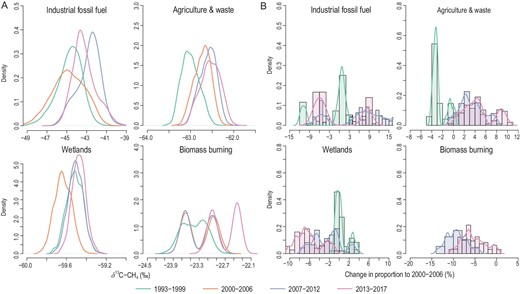
\includegraphics[width=\textwidth, height=9cm]{figure 3.jpeg}
    \label{fig3:my_label}


\textit{\scriptsize{Changes in $\delta^{13}$$C-CH_{4}$ values and in contribution of $^{13}CH_{4}$ mass to the annual total of $^{13}CH_{4}$ mass for major source categories during 1993–2017. (A) Density function of the mean emission-weighted $\delta^{13}$$C-CH_{4}$ value of the sources for four time periods from Monte Carlo accounting (n=96000):decreased atmospheric growth during 1993-1999, relative stabilization during 2000-2006, renewed growth during 2007-2012 and accelerated growth during 2013-2017. While the emission-weighted $\delta^{13}$$C-CH_{4}$ signatures may change over time, it is the combination of these signatures with their respective emission amounts that determines the atmospheric isotopic trend. (B) Density distribution of changes in the contribution of $^{13}CH_{4}$ mass from major $CH_{4}$ mass in the source during 1993-1999, 2007-2012 and 2013-2017 relative to the $CH_{4}$ plateau period 2000-2006.}}
\end{figure}
\\\\
\small{The change in the $\delta^{13}$$C-CH_{4}$ contribution from individual sources does not necessarily imply the same trend in the global average signature. Theoretically, even if the tropical wetland signature becomes more positive, the increased proportion of wetland-contributed $^{13}CH_{4}$ mass to the total $^{13}CH_{4}$ mass can still result in a shift towards a more negative global signal, as the biogenic signature is considerably lighter than the global atmospheric $\delta^{13}$$C-CH_{4}$ value [36] $(\sim-53.6\%)$ before fractionation. This is the case in some paleoclimate studies [52] where tropical wetlands and other natural sources (e.g. biomass burning) dominated the annual $CH_{4}$ budget. However, the role of human activities has become dominant in the annual $CH_{4}$ and isotope budgets since AD 1750, and the relative importance of wetlands has lessened. Figure \ref{fig3:my_label}B also shows the probability distribution of the relative contribution of $^{13}CH_{4}$ mass to the annual total $^{13}CH_{4}$mass in the source, from 2000–2006 to the post-2007 period.$IFF_{CH4}$ exhibits either an increased contribution of $5\%-8\%$ based on EDGARv4.2 or a decreased contribution of $6\%-9\%$ relative to 2000-2006 based on SCH150 or GAINS. In contrast to $IFF_{CH4}$, $AGW_{CH4}$ shows a significantly increasing contribution to the isotope budget from 2000-2006 to the post-2007 period, with a positive trend of $5\%-7\%$ relative to 1993-1999. This pattern can be explained by the substantial increase in $AGW_{CH4}$ production since the 21st century. The contribution of $BB_{CH4}$ to the $^{13}CH_{4}$ mass was $20\%-25\%$ lower in 2007-2017 than in 1993-1999 and 2000-2006, mainly due to reduced biomass burning, as suggested by the inversion model based on satellite retrievals [13] and by inventories [47].}






\subsection*{\textbf{\textsc{\large{Idealized wetland emission scenarios that reproduce the decrease in atmospheric $\delta^{13}$$C-CH_{4}$ values}}}}  


\small{Beyond our wetland-model ensemble, we created scenarios to investigate the possible involvement of rising WET${CH4}$ in the decrease of atmospheric $\delta^{13}$$C-CH{4}$ values. To do so, we performed a sensitivity test by running the box model in inverse mode for each individual run to calculate idealized WET${CH4}$ given the other sources, varying OH concentration, atmospheric CH4 and δ13C-CH4 observations, and the isotopic signatures of the sources, which thus linearizes the problem. The results suggest that the magnitude of increase in idealized WET${CH4}$ largely depends on the hypothesis of IFF sources, where greater wetland increases are required to compensate for the large increase in the IFF${CH4}$ scenarios (Fig. \ref{fig4:my_label}A). Note that all the idealized WET${CH4}$ scenarios are higher than the two WET${CH4}$ scenarios in this study (i.e. CRU and REN) or WetCHARTs, a wetland ${CH4}$ product that is based on satellite-derived surface water extent and precipitation reanalysis and an ensemble of ecosystem respiration estimates. One process-based WET${CH4}$ that overlaps the increases in idealized wetland scenarios is the ensemble mean of LPJ-wsl simulations for a future projection under the climate scenario RCP8.5 [53] (denoted Zhang2017). RCP8.5 is considered the upper bound of wetland CH4 feedback to rising temperature in LPJ-wsl because the strong and steady increase in temperature in RCP8.5 is higher than that determined from actual observations. Note that this scenario would occur only in combination with the hypothesis that IFF${CH4}$ has had no significant trends in recent years.}

\newpage
\begin{figure}[H]
    \caption{}
    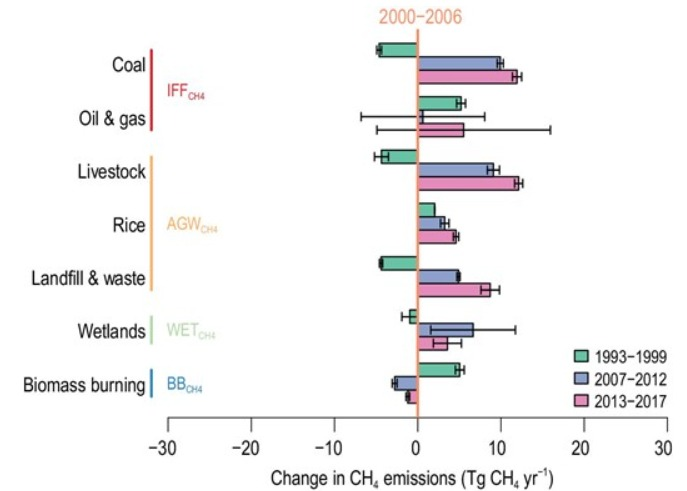
\includegraphics[width=\textwidth, height=9cm]{figure 4.png}
    \label{fig4:my_label}
   
    
\textit{\scriptsize{Idealized wetland emissions that reproduce the observations of atmospheric CH4 and δ13C-CH4 for 2000–2017. (A) Time series of anomalies of idealized WET${CH4}$ with a 7-year moving window (colored lines: ensemble mean grouped by IFF${CH4}$) in comparison to the two emission scenarios (CRU and REN) applied in this study and the estimates from Ref. [53] (denoted Zhang2017) and WetCHARTs [41]. All estimates are anomalies relative to 2001. The min/max range of idealized wetland emissions is shown as the gray area. (B) Trend of wetland emissions for 2000–2017 computed using linear regression. Significant trends at the 95\% confidence level are denoted with.}}
\end{figure}
\\

\small{The comparison of 2000–2017 trends in WET${CH4}$ (Fig. \ref{fig4:my_label}B) suggests that to reproduce the magnitude of the observed decrease in atmospheric $\delta^{13}$$C-CH{4}$ values, the required emission increase from natural wetlands would need to be much higher than the current estimates from process-based wetland models. The trend of CRU is consistent with the ensemble estimate of global wetland model simulations [5,40], while that of REN is at the higher end of the trends that consider the potential inundation increase due to enhanced tropical precipitation [22]. Note that the range of idealized increases in WET${CH4}$ is in line with two recent inversion studies [8,10] based on GOSAT $CH^{4}$ measurements, which suggests a positive wetland trend of 2–3 Tg $CH_^{4}$ yr–1 yr–1 for 2010–2018. However, to produce such a significant trend, the Q10 parameter (temperature sensitivity of $CH_^{4}$ emissions) in the wetland models would need to be much higher than the range of 2–3 from LPJ-wsl and WetCHARTs or the measurement-based average of 2.57 from FLUXNET-$CH_^{4}$ [54]. In addition, a recent multi-model ensemble inversion study [55] suggests that the observation-constrained wetland $CH_^{4}$ feedback to rising temperature is lower than that of Zhang 2017. Despite this, there are considerable uncertainties in modeled WET${CH4}$ due to scarcity of measurements for the tropics [40]. We conclude that the hypothesis that a large increase in natural wetlands drives the decrease in atmospheric $\delta^{13}$$C-CH{4}$ values cannot be reconciled with process-based wetland $CH_^{4}$ models.}

\newpage
\subsection*{\textbf{\textsc{\large{Attributions of the $CH_^{4}$ rise based on the most likely scenarios}}}}

\small{Our Monte Carlo estimation (Table 1) suggests that the largest uncertainties in global representative source $\delta^{13}$$C-CH_{4}$ values are in industrial fossil fuel activities, providing clues for future studies. Our estimated global representative values for total $CH_^{4}$ source signatures are within the uncertainty of recently compiled databases [12,36] but are lower than the value used in previous inverse studies (see Fig. S6 for references). Among the major $CH_^{4}$ emission sectors, the global average emission-weighted $\delta^{13}$$C-CH_{4}$ signature for coal has the highest IAV, which is mainly due to the large deviation in country-level data in coal emissions [39] and the heterogeneous distribution of different coal ranks [56]. Note that the low-rank coals tend to produce isotopically lighter $CH_^{4}$ [36] with a potentially biogenic origin [57], indicating that the proportion of consumption of different coal types may have a significant impact on atmospheric $\delta^{13}$$C-CH_{4}$ values.}\\

\textit{\scriptsize{\textbf{Table 1.}Statistics of global representative average $\delta^{13}$$C-CH_{4}$ values for the major CH4 categories used in the Monte Carlo simulations for 1993–2017. The interannual variability (IAV), uncertainty propagated from bottom-up estimates, and the full uncertainty that considers both uncertainty from emissions and spatially resolved distribution of source signatures for different $CH_^{4}$ categories are listed. See Table S2 for $CH_^{4}$ sectors that are not shown here.}}\\
   
  \begin{center}
      \begin{tabular}{| c | c | c | c | | c | }
      \hline
       \multicolumn{5}{ |c| }{Tabla 1} \\ \hline
       $\delta^{13}$$C-CH_{4}$ (‰) & 	Mean & IAV	&  Uncertainty from emissions & Full uncertainty \\ \hline
        Coal &  $-45.8$ & 0.71 & 1.23 & 2.57 \\
        Oil \& gas  & $-43.8$  & 0.06  & 0.61 & 0.93  \\
        Livestock  & $-65.4$ & 0.16  & 0.32 & 0.86  \\
        Wetlands  & $-59.6$  & 0.10  & 0.15 & 0.20  \\ 
        Biomass burning^a & $-23.9$ & 0.38 & 0.03 & 0.14 \\
        \hline
      \end{tabular}
      \caption{Statistics of global}
      \label{tab1: 1}
     \end{center}\\
\textit{\scriptsize{$^a$The higher IAV of $BB_{CH_4}$ than the uncertainty range is due to the spikes during some extreme El Niño years, which are one order of magnitude higher than that of most years.}}\\
    
\small{We calculate the most likely scenarios based on the agreement of bottom-up estimates with isotopic observations (Fig. \ref{fig5:my_label}). The results suggest that the agricultural, landfill and waste sectors account for 53 ± 13\% (21.0 ± 0.8 Tg $CH_^{4}$ yr–1; 1-σ) of renewed growth over the period of 2007–2017 compared to 2000–2006, with industrial fossil fuel sources and wetland sources contributing 34 ± 24\% (13.7 ± 8.8 Tg $CH_^{4}$ yr–1) and 13 ± 9\% (5.3 ± 3.5 Tg $CH_^{4}$ yr–1), respectively. The decreasing emissions from fossil fuel sectors in 1993–1999 compared to 2000–2006, combined with the increasing OH anomaly (Fig. S8), may have contributed to the $CH_^{4}$ stabilization period (Fig. \ref{fig5:my_label} and Fig. S7). The increases in methane emissions (mainly from the fossil fuel, agriculture and waste sectors) combined with a step increase from wetland $CH_^{4}$ and small decreases in OH levels led to renewed growth in methane during 2007–2012. Moreover, the higher $CH_^{4}$ emissions from mainly anthropogenic activities, i.e. coal, oil, gas, livestock, landfill and waste sectors, drove the accelerated increase in atmospheric $CH_^{4}$ during 2013–2017. These sectoral emission increases are consistent with economic activity data (Table S2; Table S3) showing that, in the past decade, coal production has increased by 41.7\% globally (International Energy Agency,https://www.iea.org/topics/coal/statistics/) and that the populations of major livestock species (e.g. swine, chickens and ruminant animals) have increased by 22.5\% (FAOSTAT, http://www.fao.org/faostat/). Although coal production exhibited a temporary decline during 2014–2016 (Statistical Review of World Energy 2020,https://www.bp.com/content/dam/bp/business-sites/en/global/corporate/pdfs/energy- \\economics/statistical-review/bp-stats-review-2020-full-report.pdf), average coal emissions during 2013–2017 were higher than those during 2007–2012, indicating that coal mining emissions continued to grow, with a higher contribution to the increase in atmospheric $CH_^{4}$.}
  
\begin{figure}[H]
    \caption{}
    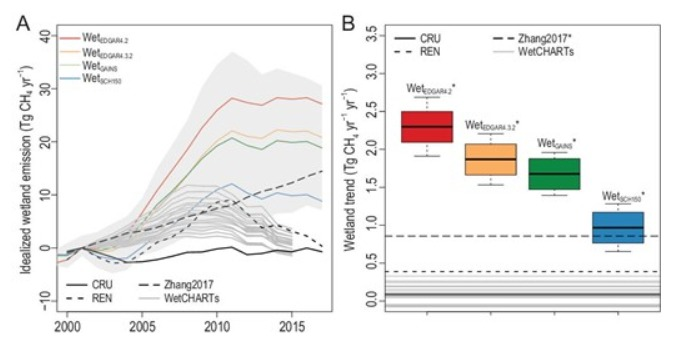
\includegraphics[width=\textwidth, height=9cm]{figure 5.png}
    \label{fig5:my_label}

\textit{\scriptsize{Changes in average total $CH_^{4}$ emissions in the most likely scenarios. The changes in $CH_^{4}$ emissions over the three periods are calculated relative to the average in the$CH_^{4}$ plateau period 2000–2006 (vertical reference line in orange). The most likely scenarios are defined as the subset of emission scenarios (n = 960) in the first percentile lowest mean squared difference (MSD) (Fig. S6) in comparison to the full ensembles (n = 96\ 000; Fig. S9). IFF $CH_^{4}$, AGWCH4, WET${CH4}$ and BBCH4 represent the $CH^{4}$ sectors of industrial fossil fuels, agriculture and waste, wetlands, and biomass burning, respectively.}}
\end{figure}

\section*{\textbf{\textsc{\Large{\underline{CONCLUSIONS}}}}}

\small{Our analysis shows that a comprehensive evaluation of hypotheses regarding the attribution of rising atmospheric $CH_{4}$ based on a combination of bottom-up approaches and isotopic values can reconcile multiple lines of evidence into a robust global $CH_{4}$ budget. However, we acknowledge that there are some biases and uncertainties in the bottom-up estimates and that our exploration of possible emission scenarios does not cover all potential scenarios. This study clearly suggests that the proposed hypotheses are influenced by the choice of a priori estimates, indicating that the high-bias a priori estimates of trends applied in some earlier studies have led to equally biased conclusions regarding the attribution of atmospheric methane rise. Our results suggest that decreasing emissions from coal, oil and gas from 1993–1999 to 2000–2006, combined with the increasing OH anomaly, likely contributed to the methane stabilization period. Anthropogenic sources were the most likely major contributor to the renewed growth in $CH_{4}$ after 2006. Moreover, the good agreement of low present-day geological source estimates with observations supports the hypothesis that the IFF$CH_{4}$ in recent decades has been largely underestimated. However, our understanding of the role of livestock and wetlands, particularly in tropical regions, is more limited. Aircraft measurements in these regions may help address the lack of data and improve our understanding of WET$CH_{4}$. This study highlights the dominant role of anthropogenic emissions from fossil fuels, agriculture, landfills and waste in driving the recent rising trend in atmospheric $CH_{4}$. Our findings improve our understanding of the causes of changes in atmospheric $CH_{4}$ over the past 25 years, enabling the development of more targeted mitigation strategies and policies to stabilize and ultimately reduce key contributing emission sectors.}

\section*{\textbf{\textsc{\Large{\underline{MATERIALS AND METHODS}}}}}

\subsection*{\textbf{\textsc{\large{Model descriptions}}}}\\

\small{The model was developed from previous studies [15,60,61] and consists of two perfectly mixed boxes representing the troposphere in the northern and southern hemispheres. The changes in $CH_4$ concentration are calculated using the following equations:}

 \begin{equation}
    \label{1}
        ^{12}CH_4^N(t+\Delta t) = {^{12}}CH_4^N(t)+\Biggl(\dst\sum_{i} {^{12}}S_i^N(t)+\dst\sum_{j} k_j^{{12}^{12}}CH_4^N(t)-\frac{1}{2\tau_{ex}} {^{12}}CH_4^N(t)+\frac{1}{2\tau_{ex}} {^{12}}CH_4^S(t)\Biggr)\Delta t,
    \end{equation}

\begin{equation}
    \label{2}
        ^{12}CH_4^S(t+\Delta t) = {^{12}}CH_4^S(t)+\Biggl(\dst\sum_{i} {^{12}}S_i^S(t)+\dst\sum_{j} k_j^{{13}^{12}}CH_4^S(t)-\frac{1}{2\tau_{ex}} {^{12}}CH_4^S(t)+\frac{1}{2\tau_{ex}} {^{12}}CH_4^N(t)\Biggr)\Delta t.
    \end{equation}

\small{where $^{12}CH_4$ is approximated by $CH_4$ and $^{12}S_i^N(t)$ and $^{12}S_i^S(t)$ represent the annual source strength of the source in the northern hemisphere and southern hemisphere, respectively. $k^{12}$ is the first-order removal rate coefficient for the sinks. The interhemispheric exchange time τ is set to a constant value of 1 yr given that the overall methane $CH_4$ concentration and $OH$ anomalies are largely unaffected by the interhemispheric exchanges [15].}
\\\\\
\small{The $\delta^{13}C-CH_4$ isotopic signatures of the different source categories i and the kinetic isotope effect (KIE) in the individual sink reactions j are used to calculate the sources $({^{13}}S_i)$ and removal rate coefficients $({^{13}}k_j)$ for $\delta^{13}C-CH_4$ values.}
\\\\
\small{These terms are then used to derive the mixing ratio changes in $^{13}C-CH_4$:}

\begin{equation}
    \label{3}
        ^{13}CH_4^N(t+\Delta t) = {^{13}}CH_4^N(t)+\Biggl(\dst\sum_{i} {^{13}}S_i^N(t)+\dst\sum_{j} k_j^{{13}^{13}}CH_4^N(t)-\frac{1}{2\tau_{ex}} {^{13}}CH_4^N(t)+\frac{1}{2\tau_{ex}} {^{13}}CH_4^S(t)\Biggr)\Delta t,
    \end{equation}

\begin{equation}
    \label{4}
        ^{13}CH_4^S(t+\Delta t) = {^{13}}CH_4^S(t)+\Biggl(\dst\sum_{i} {^{13}}S_i^S(t)+\dst\sum_{j} k_j^{{13}^{13}}CH_4^S(t)-\frac{1}{2\tau_{ex}} {^{12}}CH_4^S(t)+\frac{1}{2\tau_{ex}} {^{13}}CH_4^N(t)\Biggr)\Delta t.
    \end{equation}

\small{The mixing ratios of the individual isotopologues are converted to $\delta$ values as follows:}

\begin{equation}
    \label{5}
        \delta_C^{13}=\Biggl(\frac{ ^{13}CH_4/ {^{12}}CH_4}{ ^{13}R_{std}}-1\Biggr),
    \end{equation}

\small{where $^{13}R_{std} = 1.12372\%$ is the $^{13}C/{^{12}C$ ratio of the international reference material Vienna Pee Dee Belemnite (VPDB).}
\\\\
\small{The soil sink is considered to have a low IAV, as suggested by biogeochemical models [62,63], despite a recent study [64] based on a few site-level measurements suggesting a decline in the soil sink in temperate forests in recent decades. For soil $CH_4$ uptake, we use climatology from a process-based model [63] in the calculation of the hemispheric net $CH_4$ source (see equation \ref{6} in Materials and Methods). The contributions of $Cl$ sink and stratospheric loss to the removal of $CH_4$ in the troposphere are highly uncertain and not well constrained by direct observations, but have a strong kinetic isotope effect on ${^{13}}CH_4$. Given the large uncertainty in $Cl$ and stratospheric sinks and the lack of available datasets, the magnitudes of these two sinks were not explicitly considered in the calculation of the hemispheric $CH_4$ budget. We assume that the annual methane removal rate is driven solely by OH variability, while other minor sinks are kept constant over the study period. Because sensitivity tests [65] suggest that the uncertain magnitude of $Cl$ fields leads to a wide range of simulated $\delta^{13}C-CH_4$ values given its strong ‘isotope leverage’ effect [66] $(−60 \pm 1\%)$ on total $\epsilon$, the sink-weighted average fractionation factor $\epsilon$ is highly uncertain. The approach in this study is to estimate the total $\varepsilon$ value for each box model run that optimizes the match between atmospheric observations and simulation at the onset of the study period. The optimized $\varepsilon$ values were derived from running the box model in inverse mode by matching the observed global average [11]. This allows us to explore the uncertainty in $\varepsilon$ based on bottom-up source aggregation and the uncertainty in $\delta^{13}C-CH_4$ values. Figure S6 shows that the estimated fractionation factors for the full ensemble and first percentile ensemble are broadly in agreement with previous studies [11–13,60,66–70]. The distribution of the mean methane lifetime (Fig. S9) over the study period is slightly lower than the estimated $9.1 \pm 0.9$ yr from Ref. [71] and is comparable in magnitude to that between atmospheric chemistry-transport models in the recent model intercomparison [31,32,72]. Here, we evaluate the global results from the box model, instead of hemispheric results, to minimize the potential influence of uncertainty in IAV from interhemispheric transport on box model performance, as suggested by a recent study [73]. See Supplementary Data for details about the model strategy.}

\subsection*{\textbf{\textsc{\large{$CH_4$ source estimates}}}}\\

\small{To test all the proposed competing hypotheses, we carried out simulation experiments using box modeling for different emission scenarios based on a suite of bottom-up datasets. We first list all the possible options for the $CH_4$ inventories by five $CH_4$ source categories (i.e. $IFF_{CH_4}$, $AGW_{CH_}4$, $WET_{CH_}4$, $BB_{CH_4}$ and $GEO_{CH_4}$) and then generate emission scenarios with combinations of $CH_4$ inventories. The assignment of the inventory (i.e. $EDGAR$)-specific sectors into the main categories $IFF_{CH_4}$, $AGW_{CH_4}$ and $BB_{CH_4}$ follows the criteria from Supplementary Table S4 in Ref. [5]. Anthropogenic $CH_4$ emissions related to fossil fuels from exploitation, transportation and usage of coal, oil and natural gas are defined as $IFF_{CH_4}$. For methane sectors related to enteric fermentation and manure, landfills, waste and rice agriculture are defined as $AGW_{CH_4}.}

\subsection*{\textbf{\textsc{\large{Spatially resolved $\delta^{13}C-CH_4$ and uncertainty estimation}}}}\\

\small{Spatially resolved distributions of $\delta^{13}C-CH_4$ source signatures for the following major methane categories were applied in this study: coal, natural gas/oil, livestock, wetlands and biomass burning. For the other sources, including agricultural waste, rice, geological sources, termites, freshwater systems and wild animals, we use a globally averaged value (Table S4) from a global inventory database that collected isotopic source signatures based on literature values [36,66,68].}

\subsection*{\textbf{\textsc{\large{Emission scenarios}}}}\\

\small{An emission scenario is a combination of the individual $CH_4$ source estimates listed in Table S1. Annual total net $CH_4$ sources can be expressed as follows:}
\begin{equation}
    \label{6}
        S_{tot}=S_{IFF}+S_{AGW}+S_{WET}+S_{BB}+S_{GEO},+S_{OTH}−S_{soil},
    \end{equation}

\small{where $S$ represents the individual $CH_4$ source from Table S1 and $S_{soil}$ is a constant soil sink. The total number of emission scenarios is 96, calculated as 4 $IFF_{CH_4} \times 3 AWG_{CH_4} × 2 WET_{CH_4} × \\2 BB_{CH_4} × 2 GEO_{CH_4}$. For each emission scenario, we use Monte Carlo techniques to estimate the uncertainty in the source signature propagated from bottom-up estimates and the spatial variability of the source signature. A set of 1000 random maps of $\delta^{13}C-CH_4$ values for each major $CH_4$ source (Table 1) were generated based on the uncertainty maps in this study assuming a Gaussian distribution. For $CH_4$ sources that are not spatially resolved, 1000 samples of the global-representative signature values are calculated with mean and 1-standard deviation defined by observations from the compiled databases (Table S4). One thousand sets of emission-weighted hemispheric time series of $\delta^{13}C-CH_4$, which were calculated with bottom-up estimates depending on emission scenarios, were used as inputs for the box model. For each emission scenario, the simulated time series of $\delta^{13}C-CH_4$ values covers the uncertainty range of spatial variability in the isotopic signatures of major $CH_4$ categories.}


\section*{\textbf{\textsc{\Large{\underline{DATA AVAILABILITY}}}}}

\small{All data needed to evaluate the conclusions in this paper are present in the paper and/or the Supplementary Data. Additional ancillary data are available from the corresponding author upon request.}

\section*{\textbf{\textsc{\Large{\underline{Acknowledgements}}}}}

\small{We thank A.J. Turner for sharing the basis of our box model, G. Janssens-Maenhout et al. for sharing the EDGAR inventories and O. Sherwood for sharing the database of $\delta^{13}C-CH_4$ signatures. We thank S. Schwietzke, N. Chandra and S. Strode for their constructive comments. J.G.C. and A.S. are grateful for the support of the Australian National Environmental Science Program-Earth Systems and Climate Change Hub. We thank the University of Colorado's Institute of Arctic and Alpine Research (INSTAAR) (https://instaar.colorado.edu) and National Oceanic and Atmospheric Administration (NOAA) Earth System Research Laboratory (ESRL) (https://www.esrl.noaa.gov) for sharing the atmospheric $\delta^{13}C-CH_4$ measurements.}

\section*{\textbf{\textsc{\Large{\underline{FUNDING}}}}}

\small{We acknowledge support from the Strategic Priority Research Program of the Chinese Academy of Sciences (XDA19040504 and XDA19070204) and the Gordon and Betty Moore Foundation through grant GBMF5439 ‘Advancing Understanding of the Global Methane Cycle’ supporting the Methane Budget released by the Global Carbon Project (globalcarbonproject.org). P.K.P. is partly supported by the Environment Research and Technology Development Fund (JPMEERF20182002) of the Environmental Restoration and Conservation Agency of Japan.}

\textbf{Conflict of interest statement.} \small{None declared.}

\begin{thebibliography}{}
\begin{enumerate}
    \item	Ocko IB, Sun T, Shindell D et al.  Acting rapidly to deploy readily available methane mitigation measures by sector can immediately slow global warming. Environ Res Lett 2021; 16: 054042.10.1088/1748-9326/abf9c8
    Google ScholarCrossrefWorldCat 
    \item	Meinshausen M, Vogel E, Nauels A et al.  Historical greenhouse gas concentrations for climate modelling (CMIP6). Geosci Model Dev 2017; 10: 2057–116. 10.5194/gmd-10-2057-2017
    Google ScholarCrossrefWorldCat 
    \item	Nisbet EG, Manning MR, Dlugokencky EJ et al.  Very strong atmospheric methane growth in the 4 years 2014–2017: implications for the Paris Agreement. Glob Biogeochem Cycles 2019; 33: 318–42. doi: agupubs.onlinelibrary.wiley.com/doi/full/10.1029/2018GB006009
    Google ScholarCrossrefWorldCat 
    \item	Ferretti DF. Unexpected changes to the global methane budget over the past 2000 years. Science 2005; 309: 1714–7. 10.1126/science.1115193
    Google ScholarCrossrefPubMedWorldCat 
    \item	Saunois M, Stavert AR, Poulter B et al.  The global methane budget 2000–2017. Earth Syst Sci Data 2020; 12: 1561–623. 10.5194/essd-12-1561-2020
    Google ScholarCrossrefWorldCat 
    \item	Nisbet EG, Dlugokencky EJ, Bousquet P. Methane on the rise—again. Science 2014; 343: 493–5. 10.1126/science.1247828
    Google ScholarCrossrefPubMedWorldCat 
    \item	Thompson RL, Nisbet EG, Pisso I et al.  Variability in atmospheric methane from fossil fuel and microbial sources over the last three decades. Geophys Res Lett 2018; 45: 11499–508. 10.1029/2018GL078127
    Google ScholarCrossrefWorldCat 
    \item	Yin Y, Chevallier F, Ciais P et al.  Accelerating methane growth rate from 2010 to 2017: leading contributions from the tropics and East Asia. Atmos Chem Phys 2021; 21: 12631–47. 10.5194/acp-21-12631-2021
    Google ScholarCrossrefWorldCat 
    \item	He J, Naik V, Horowitz LW et al.  Investigation of the global methane budget over 1980–2017 using GFDL-AM4.1. Atmos Chem Phys 2020; 20: 805–27. 10.5194/acp-20-805-2020
    Google ScholarCrossrefWorldCat 
    \item	Zhang Y, Jacob DJ, Lu X et al.  Attribution of the accelerating increase in atmospheric methane during 2010–2018 by inverse analysis of GOSAT observations. Atmos Chem Phys 2021; 21: 3643–66. 10.5194/acp-21-3643-2021
    Google ScholarCrossrefWorldCat 
    \item	Schaefer H, Fletcher SEM, Veidt C et al.  A 21st-century shift from fossil-fuel to biogenic methane emissions indicated by 13CH4. Science 2016; 352: 80–4. 10.1126/science.aad2705
    Google ScholarCrossrefPubMedWorldCat 
    \item	Schwietzke S, Sherwood OA, Bruhwiler LMP et al.  Upward revision of global fossil fuel methane emissions based on isotope database. Nature 2016; 538: 88–91. 10.1038/nature19797
    Google ScholarCrossrefPubMedWorldCat 
    \item	Worden JR, Bloom AA, Pandey S et al.  Reduced biomass burning emissions reconcile conflicting estimates of the post-2006 atmospheric methane budget. Nat Commun 2017; 8: 2227.10.1038/s41467-017-02246-0
    Google ScholarCrossrefPubMedWorldCat 
    \item	Rigby M, Montzka SA, Prinn RG et al.  Role of atmospheric oxidation in recent methane growth. Proc Natl Acad Sci USA 2017; 114: 5373–7. 10.1073/pnas.1616426114
    Google ScholarCrossrefPubMedWorldCat 
    \item	Turner AJ, Frankenberg C, Wennberg PO et al.  Ambiguity in the causes for decadal trends in atmospheric methane and hydroxyl. Proc Natl Acad Sci USA 2017; 114: 5367–72. 10.1073/pnas.1616020114
    Google ScholarCrossrefPubMedWorldCat 
    \item	Saunois M, Bousquet P, Poulter B et al.  Variability and quasi-decadal changes in the methane budget over the period 2000–2012. Atmos Chem Phys 2017; 17: 11135–61. 10.5194/acp-17-11135-2017
    Google ScholarCrossrefWorldCat 
    \item	Turner AJ, Frankenberg C, Kort EA. Interpreting contemporary trends in atmospheric methane. Proc Natl Acad Sci USA 2019; 116: 2805–13. 10.1073/pnas.1814297116
    Google ScholarCrossrefPubMedWorldCat 
    \item	Nisbet EG, Fisher RE, Lowry D et al.  Methane mitigation: methods to reduce emissions, on the path to the Paris Agreement. Rev Geophys 2020; 58: e2019RG000675.10.1029/2019RG000675
    Google ScholarCrossrefWorldCat 
    \item	Nisbet EG, Dlugokencky EJ, Manning MR et al.  Rising atmospheric methane: 2007–2014 growth and isotopic shift: rising methane 2007–2014. Glob Biogeochem Cycles 2016; 30: 1356–70. 10.1002/2016GB005406
    Google ScholarCrossrefWorldCat 
    \item	Wolf J, Asrar GR, West TO. Revised methane emissions factors and spatially distributed annual carbon fluxes for global livestock. Carbon Balance Manage 2017; 12: 16.10.1186/s13021-017-0084-y
    Google ScholarCrossrefWorldCat 
    \item	Lunt MF, Palmer PI, Feng L et al.  An increase in methane emissions from tropical Africa between 2010 and 2016 inferred from satellite data. Atmos Chem Phys 2019; 19: 14721–40. 10.5194/acp-19-14721-2019
    Google ScholarCrossrefWorldCat 
    \item	Zhang Z, Zimmermann NE, Calle L et al.  Enhanced response of global wetland methane emissions to the 2015–2016 El Niño-Southern Oscillation event. Environ Res Lett 2018; 13: 074009.10.1088/1748-9326/aac939
    Google ScholarCrossrefPubMedWorldCat 
    \item	Janssens-Maenhout G, Crippa M, Guizzardi D et al.  EDGAR v4.3.2 Global Atlas of the three major greenhouse gas emissions for the period 1970–2012. Earth Syst Sci Data 2019; 11: 959–1002. 10.5194/essd-11-959-2019
    Google ScholarCrossrefWorldCat 
    \item	Höglund-Isaksson L. Bottom-up simulations of methane and ethane emissions from global oil and gas systems 1980 to 2012. Environ Res Lett 2017; 12: 024007.10.1088/1748-9326/aa583e
    Google ScholarCrossrefWorldCat 
    \item	Helmig D, Rossabi S, Hueber J et al.  Reversal of global atmospheric ethane and propane trends largely due to US oil and natural gas production. Nat Geosci 2016; 9: 490–5. 10.1038/ngeo2721
    Google ScholarCrossrefWorldCat 
    \item	Dalsøren SB, Myhre G, Hodnebrog Ø et al.  Discrepancy between simulated and observed ethane and propane levels explained by underestimated fossil emissions. Nat Geosci 2018; 11: 178–84. 10.1038/s41561-018-0073-0
    Google ScholarCrossrefWorldCat 
    \item	Petrenko VV, Smith AM, Schaefer H et al.  Minimal geological methane emissions during the Younger Dryas–Preboreal abrupt warming event. Nature 2017; 548: 443–6. 10.1038/nature23316
    Google ScholarCrossrefPubMedWorldCat 
    \item	Hmiel B, Petrenko VV, Dyonisius MN et al.  Preindustrial 14CH4 indicates greater anthropogenic fossil CH4 emissions. Nature 2020; 578: 409–12. 10.1038/s41586-020-1991-8
    Google ScholarCrossrefPubMedWorldCat 
    \item	Etiope G, Ciotoli G, Schwietzke S et al.  Gridded maps of geological methane emissions and their isotopic signature. Earth Syst Sci Data 2019; 11: 1–22. 10.5194/essd-11-1-2019
    Google ScholarCrossrefWorldCat 
    \item	Naik V, Voulgarakis A, Fiore AM et al.  Preindustrial to present-day changes in tropospheric hydroxyl radical and methane lifetime from the Atmospheric Chemistry and Climate Model Intercomparison Project (ACCMIP). Atmos Chem Phys 2013; 13: 5277–98. 10.5194/acp-13-5277-2013
    Google ScholarCrossrefWorldCat 
    \item	Nicely JM, Canty TP, Manyin M et al.  Changes in global tropospheric OH expected as a result of climate change over the last several decades. J Geophys Res Atmos 2018; 123: 10774–95. doi: agupubs.onlinelibrary.wiley.com/doi/full/10.1029/2018GB006009
    Google ScholarCrossrefWorldCat 
    \item	Zhao Y, Saunois M, Bousquet P et al.  Inter-model comparison of global hydroxyl radical (OH) distributions and their impact on atmospheric methane over the 2000–2016 period. Atmos Chem Phys 2019; 19: 13701–23. 10.5194/acp-19-13701-2019
    Google ScholarCrossrefWorldCat 
    \item	Naus S, Montzka SA, Patra PK et al.  A three-dimensional-model inversion of methyl chloroform to constrain the atmospheric oxidative capacity. Atmos Chem Phys 2021; 21: 4809–24. 10.5194/acp-21-4809-2021
    Google ScholarCrossrefWorldCat 
    \item	Patra PK, Krol MC, Prinn RG et al.  Methyl chloroform continues to constrain the hydroxyl (OH) variability in the troposphere. J Geophys Res Atmos 2021; 126: e2020JD033862.
    Google ScholarCrossrefWorldCat 
    \item	Naus S, Montzka SA, Pandey S et al.  Constraints and biases in a tropospheric two-box model of OH. Atmos Chem Phys 2019; 19: 407–24. 10.5194/acp-19-407-2019
    Google ScholarCrossrefWorldCat 
    \item	Sherwood OA, Schwietzke S, Arling VA et al.  Global inventory of gas geochemistry data from fossil fuel, microbial and burning sources, version 2017. Earth Syst Sci Data 2017; 9: 639–56. 10.5194/essd-9-639-2017
    Google ScholarCrossrefWorldCat 
    \item	Feinberg AI, Coulon A, Stenke A et al.  Isotopic source signatures: impact of regional variability on the δ13CH4 trend and spatial distribution. Atmos Environ 2018; 174: 99–111. 10.1016/j.atmosenv.2017.11.037
    Google ScholarCrossrefWorldCat 
    \item	Ganesan AL, Stell AC, Gedney N et al.  Spatially resolved isotopic source signatures of wetland methane emissions. Geophys Res Lett 2018; 45: 3737–45. 10.1002/2018GL077536
    Google ScholarCrossrefWorldCat 
    \item	Miller SM, Michalak AM, Detmers RG et al.  China's coal mine methane regulations have not curbed growing emissions. Nat Commun 2019; 10: 303.10.1038/s41467-018-07891-7
    Google ScholarCrossrefPubMedWorldCat 
    \item	Poulter B, Bousquet P, Canadell JG et al.  Global wetland contribution to 2000–2012 atmospheric methane growth rate dynamics. Environ Res Lett 2017; 12: 094013.10.1088/1748-9326/aa8391
    Google ScholarCrossrefWorldCat 
    \item	Bloom AA, Bowman KW, Lee M et al.  A global wetland methane emissions and uncertainty dataset for atmospheric chemical transport models (WetCHARTs version 1.0). Geosci Model Dev 2017; 10: 2141–56. 10.5194/gmd-10-2141-2017
    Google ScholarCrossrefWorldCat 
    \item	Taylor KE. Summarizing multiple aspects of model performance in a single diagram. J Geophys Res Atmos 2001; 106: 7183–92. 10.1029/2000JD900719
    Google ScholarCrossrefWorldCat 
    \item	Umezawa T, Brenninkmeijer CAM, Röckmann T et al.  Interlaboratory comparison of 13C and d δD measurements of atmospheric CH4 for combined use of data sets from different laboratories. Atmos Meas Tech 2018; 11:1207–31. 10.5194/amt-11-1207-2018
    Google ScholarCrossrefWorldCat 
    \item	Bruhwiler LM, Basu S, Bergamaschi P et al.  U.S. CH4 emissions from oil and gas production: have recent large increases been detected? J Geophys Res Atmos 2017; 122: 4070–83. doi: agupubs.onlinelibrary.wiley.com/doi/full/10.1029/2018GB006009
    Google ScholarCrossrefWorldCat 
    \item	Hristov AN, Harper M, Meinen R et al.  Discrepancies and uncertainties in bottom-up gridded inventories of livestock methane emissions for the contiguous United States. Environ Sci Technol 2017; 51: 13668–77. 10.1021/acs.est.7b03332
    Google ScholarCrossrefPubMedWorldCat 
    \item	Bousquet P, Ciais P, Miller JB et al.  Contribution of anthropogenic and natural sources to atmospheric methane variability. Nature 2006; 443: 439–43. 10.1038/nature05132
    Google ScholarCrossrefPubMedWorldCat 
    \item	Andela N, Morton DC, Giglio L et al.  A human-driven decline in global burned area. Science 2017; 356: 1356–62. 10.1126/science.aal4108
    Google ScholarCrossrefPubMedWorldCat 
    \item	Chang J, Peng S, Ciais P et al.  Revisiting enteric methane emissions from domestic ruminants and their δ13CCH4 source signature. Nat Commun 2019; 10: 3420.10.1038/s41467-019-11066-3
    Google ScholarCrossrefPubMedWorldCat 
    \item	McCalley CK, Woodcroft BJ, Hodgkins SB et al.  Methane dynamics regulated by microbial community response to permafrost thaw. Nature 2014; 514: 478–81. 10.1038/nature13798
    Google ScholarCrossrefPubMedWorldCat 
    \item	Sweeney C, Dlugokencky E, Miller CE et al.  No significant increase in long-term CH4 emissions on North Slope of Alaska despite significant increase in air temperature. Geophys Res Lett 2016; 43: 6604–11. 10.1002/2016GL069292
    Google ScholarCrossrefWorldCat 
    \item	Oh Y, Zhuang Q, Liu L et al.  Reduced net methane emissions due to microbial methane oxidation in a warmer Arctic. Nat Clim Chang 2020; 10: 317–21. 10.1038/s41558-020-0734-z
    Google ScholarCrossrefWorldCat 
    \item	Hopcroft PO, Valdes PJ, O’Connor FM et al.  Understanding the glacial methane cycle. Nat Commun 2017; 8: 14383.10.1038/ncomms14383
    Google ScholarCrossrefPubMedWorldCat 
    \item	Zhang Z, Zimmermann NE, Stenke A et al.  Emerging role of wetland methane emissions in driving 21st century climate change. Proc Natl Acad Sci USA 2017; 114: 9647–52. 10.1073/pnas.1618765114
    Google ScholarCrossrefPubMedWorldCat 
    \item	Delwiche KB, Knox SH, Malhotra A et al.  FLUXNET-CH4: a global, multi-ecosystem dataset and analysis of methane seasonality from freshwater wetlands. Earth Syst Sci Data 2021; 13: 3607–89. 10.5194/essd-13-3607-2021
    Google ScholarCrossrefWorldCat 
    \item	Koffi EN, Bergamaschi P, Alkama R et al.  An observation-constrained assessment of the climate sensitivity and future trajectories of wetland methane emissions. Sci Adv 2020; 6: eaay4444.10.1126/sciadv.aay4444
    Google ScholarCrossrefPubMedWorldCat 
    \item	Zazzeri G, Lowry D, Fisher RE et al.  Carbon isotopic signature of coal-derived methane emissions to the atmosphere: from coalification to alteration. Atmos Chem Phys 2016; 16: 13669–80. 10.5194/acp-16-13669-2016
    Google ScholarCrossrefWorldCat 
    \item	Vinson DS, Blair NE, Ritter DJ et al.  Carbon mass balance, isotopic tracers of biogenic methane, and the role of acetate in coal beds: powder river basin (USA). Chem Geol 2019; 530: 119329.10.1016/j.chemgeo.2019.119329
    Google ScholarCrossrefWorldCat 
    \item	Lunt MF, Palmer PI, Lorente A et al.  Rain-fed pulses of methane from East Africa during 2018–2019 contributed to atmospheric growth rate. Environ Res Lett 2021; 16: 024021.10.1088/1748-9326/abd8fa
    Google ScholarCrossrefWorldCat 
    \item	Pandey S, Houweling S, Lorente A et al.  Using satellite data to identify the methane emission controls of South Sudan's wetlands. Biogeosciences 2021; 18: 557–72. 10.5194/bg-18-557-2021
    Google ScholarCrossrefWorldCat 
    \item	Sapart CJ, Monteil G, Prokopiou M et al.  Natural and anthropogenic variations in methane sources during the past two millennia. Nature 2012; 490: 85–8. 10.1038/nature11461
    Google ScholarCrossrefPubMedWorldCat 
    \item	Tans PP. A note on isotopic ratios and the glob atmospheric methane budget. Glob Biogeochem Cycles 1997; 11: 77–81. 10.1029/96GB03940
    Google ScholarCrossrefWorldCat 
    \item	Curry CL. Modeling the soil consumption of atmospheric methane at the global scale: soil consumption of atmospheric methane. Glob Biogeochem Cycles 2007; 21: GB4012.10.1029/2006GB002818
    Google ScholarCrossrefWorldCat 
    \item	Murguia-Flores F, Arndt S, Ganesan AL et al.  Soil methanotrophy model (MeMo v1.0): a process-based model to quantify global uptake of atmospheric methane by soil. Geosci Model Dev 2018; 11: 2009–32. 10.5194/gmd-11-2009-2018
    Google ScholarCrossrefWorldCat 
    \item	Ni X, Groffman PM. Declines in methane uptake in forest soils. Proc Natl Acad Sci USA 2018; 115: 8587–90. 10.1073/pnas.1807377115
    Google ScholarCrossrefPubMedWorldCat 
    \item	Strode SA, Wang JS, Manyin M et al.  Strong sensitivity of the isotopic composition of methane to the plausible range of tropospheric chlorine. Atmos Chem Phys 2020; 20: 8405–19. 10.5194/acp-20-8405-2020
    Google ScholarCrossrefWorldCat 
    \item	Lassey KR, Etheridge DM, Lowe DC et al.  Centennial evolution of the atmospheric methane budget: what do the carbon isotopes tell us? Atmos Chem Phys 2007; 7: 2119–39. doi: acp.copernicus.org/articles/7/2119/2007/
    Google ScholarCrossrefWorldCat 
    \item	Rice AL, Butenhoff CL, Teama DG et al.  Atmospheric methane isotopic record favors fossil sources flat in 1980s and 1990s with recent increase. Proc Natl Acad Sci USA 2016; 113: 10791–6. 10.1073/pnas.1522923113
    Google ScholarCrossrefPubMedWorldCat 
    \item	Lassey KR, Ragnauth S. Balancing the global methane budget: constraints imposed by isotopes and anthropogenic emission inventories. J Integr Environ Sci 2010; 7: 97–107. 10.1080/19438151003680843
    Google ScholarCrossrefWorldCat 
    \item	Warwick NJ, Cain ML, Fisher R et al.  Using δ13C-CH4 and δD-CH4 to constrain Arctic methane emissions. Atmos Chem Phys 2016; 16: 14891–908. 10.5194/acp-16-14891-2016
    Google ScholarCrossrefWorldCat 
    \item	Monteil G, Houweling S, Dlugockenky EJ et al.  Interpreting methane variations in the past two decades using measurements of CH4 mixing ratio and isotopic composition. Atmos Chem Phys 2011; 11: 9141–53. 10.5194/acp-11-9141-2011
    Google ScholarCrossrefWorldCat 
    \item	Prather MJ, Holmes CD, Hsu J. Reactive greenhouse gas scenarios: systematic exploration of uncertainties and the role of atmospheric chemistry. Geophys Res Lett 2012; 39: L09803. 10.1029/2012GL051440
    Google ScholarWorldCatCrossref 
    \item	Nicely JM, Salawitch RJ, Canty T et al.  Quantifying the causes of differences in tropospheric OH within global models: quantifying global model OH differences. J Geophys Res Atmos 2017; 122: 1983–2007. doi: agupubs.onlinelibrary.wiley.com/doi/full/10.1029/2018GB006009
    Google ScholarCrossrefWorldCat 
    \item	Pandey S, Houweling S, Krol M et al.  Influence of atmospheric transport on estimates of variability in the global methane burden. Geophys Res Lett 2019; 46: 2302–11. 10.1029/2018GL081092
    Google ScholarCrossrefWorldCat 
\end{enumerate}
\end{thebibliography}

\end{document}